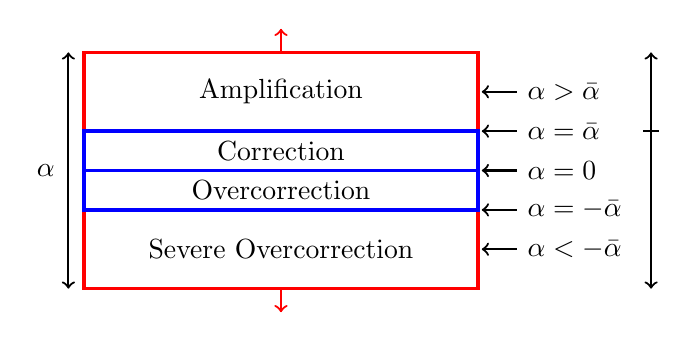
\begin{tikzpicture}
\draw[red, very thick] (-4,0) rectangle (1,1);
\draw[red, very thick] (-4,-2) rectangle (1,-1);
\draw[blue, very thick] (-4,-0.5) rectangle (1,0);
\draw[blue, very thick] (-4,-1) rectangle (1,-0.5);
%\draw[orange, ultra thick] (4,0) -- (6,0) -- (5.7,2) -- cycle;
\draw[<->,thick] (-4.2,-2) --  (-4.2,1);
\node[text width=3cm] at (-3.1,-0.5) {$\alpha$};
\draw[<-,thick] (1.05, -0.5) -- (1.5, -0.5) node [right] {$\alpha = 0$};
\draw[<-,thick] (1.05, 0) -- (1.5, 0) node [right] {$\alpha = \bar \alpha$};
\draw[<-,thick] (1.05, -1) -- (1.5, -1) node [right] {$\alpha = -\bar \alpha$};
\draw[<-,thick] (1.05, 0.5) -- (1.5, 0.5) node [right] {$\alpha > \bar \alpha$};
\draw[<-,thick] (1.05, -1.5) -- (1.5, -1.5) node [right] {$\alpha < -\bar \alpha$};
\node[text centered] at (-1.5,0.5) {Amplification};
\node[text centered] at (-1.5,-1.5) {Severe Overcorrection};
\node[text centered] at (-1.5,-0.25) {Correction};
\node[text centered] at (-1.5,-0.75) {Overcorrection};
\draw[<->,thick] (3.2,1) -- (3.2,-2);
\draw[-,thick] (3.1,0) -- (3.3,0);
\draw[red,->,thick] (-1.5,1) -- (-1.5,1.3);
\draw[red,->,thick] (-1.5,-2) -- (-1.5,-2.3);
\end{tikzpicture}